% PHẦN 1: Khối nội dung trên cùng
\noindent\hspace*{152pt}%
\begin{minipage}{380pt}
  Thay các giới hạn này vào (1), ta được
  \[
  \begin{aligned}
  f'(x) &= \lim_{h \to 0} \sin x \cdot \lim_{h \to 0} \frac{\cos h - 1}{h} + \lim_{h \to 0} \cos x \cdot \lim_{h \to 0} \frac{\sin h}{h} \\[4pt]
  &= (\sin x) \cdot 0 + (\cos x) \cdot 1 = \cos x
  \end{aligned}
  \]
  Như vậy, chúng ta đã chứng minh được công thức tính đạo hàm của hàm sin:
  \par\vspace{4pt}
  \stewartbox{2}{\frac{d}{dx} (\sin x) = \cos x}
\end{minipage}

\vspace{14pt}

% PHẦN 2: Khối giữa (Bố cục 2 cột: Hình 2 bên lề trái và Ví dụ 1 + Công thức 3 bên phải)
\noindent
\begin{minipage}[t]{130pt}
  \vspace{0pt}%
  \vspace*{18pt}% Dóng hàng tương ứng với LỜI GIẢI của Ví dụ 1
  {\small\noindent Hình 2 thể hiện đồ thị của hàm số trong Ví dụ 1 và đạo hàm của nó. Chú ý rằng $y' = 0$ bất cứ khi nào $y$ có một tiếp tuyến nằm ngang.\par}
  \vspace{8pt}
  \centering
  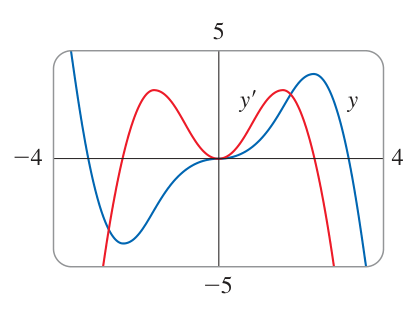
\includegraphics[width=\linewidth]{images/p0228_fig1.png}\par
  \vspace{4pt}
  {\footnotesize\textbf{HÌNH 2}}
\end{minipage}%
\hspace*{22pt}%
\begin{minipage}[t]{380pt}
  \vspace{0pt}%
  {\color{stewartBlue}\textbf{VÍ DỤ 1}}\quad Tính đạo hàm của $y = x^2 \sin x$.
  \par\vspace{6pt}
  {\color{stewartBlue}\textbf{LỜI GIẢI}}\quad Sử dụng Quy tắc nhân và Công thức 2, ta có
  \begin{align*}
  \frac{dy}{dx} &= x^2 \frac{d}{dx}(\sin x) + \sin x \frac{d}{dx}(x^2) \\[4pt]
  &= x^2 \cos x + 2x \sin x \tag*{\color{stewartBlue}\blacksquare}
  \end{align*}
  \vspace{4pt}
  Sử dụng các phương pháp tương tự như trong phép chứng minh Công thức 2, ta có thể chứng minh (xem Bài tập 26) rằng
  \par\vspace{4pt}
  \stewartbox{3}{\frac{d}{dx} (\cos x) = -\sin x}
\end{minipage}

\vspace{12pt}

% PHẦN 3: Khối dưới (Đạo hàm hàm tang và Công thức 4)
\noindent\hspace*{152pt}%
\begin{minipage}{380pt}
  Hàm tang cũng có thể được lấy đạo hàm bằng cách sử dụng định nghĩa của đạo hàm, nhưng sẽ dễ dàng hơn nếu sử dụng Quy tắc chia cùng với các Công thức 2 và 3:
  \begin{align*}
  \frac{d}{dx}(\tan x) &= \frac{d}{dx}\left(\frac{\sin x}{\cos x}\right) \\[6pt]
  &= \frac{\cos x \dfrac{d}{dx}(\sin x) - \sin x \dfrac{d}{dx}(\cos x)}{\cos^2 x} \\[6pt]
  &= \frac{\cos x \cdot \cos x - \sin x (-\sin x)}{\cos^2 x} \\[6pt]
  &= \frac{\cos^2 x + \sin^2 x}{\cos^2 x} \\[6pt]
  &= \frac{1}{\cos^2 x} = \sec^2 x \qquad \textcolor{stewartCyan}{(\cos^2 x + \sin^2 x = 1)}
  \end{align*}
  \stewartbox{4}{\frac{d}{dx} (\tan x) = \sec^2 x}
  \par\vspace{8pt}
  Đạo hàm của các hàm số lượng giác còn lại, $\csc$, $\sec$ và $\cot$, cũng có thể được tìm thấy một cách dễ dàng bằng cách sử dụng Quy tắc chia (xem Bài tập 23--25). Chúng tôi tập hợp tất cả các
\end{minipage}
